\documentclass[12pt, twoside]{article}
\usepackage[letterpaper, margin=1in, headsep=0.5in]{geometry}
\usepackage[english]{babel}
\usepackage[utf8]{inputenc}
\usepackage{amsmath}
\usepackage{amsfonts}
\usepackage{amssymb}
\usepackage{tikz}
\usetikzlibrary{quotes, angles}
\usepackage{graphicx}
\usepackage{enumitem}
\usepackage{multicol}

\newif\ifmeta
\metatrue %print standards and topics tags

\title{Regents Geometry}
\author{Chris Huson}
\date{September 2020}

\usepackage{fancyhdr}
\pagestyle{fancy}
\fancyhf{}
\renewcommand{\headrulewidth}{0pt} % disable the underline of the header
\raggedbottom


\fancyhead[LE]{\thepage}
\fancyhead[RO]{\thepage \\ Name: \hspace{4cm} \,\\}
\fancyhead[LO]{BECA / Dr. Huson / Geometry 01-Measurement\\* pset ID: 0}

\begin{document}

\subsubsection*{1-1DN-Algebra}
\begin{enumerate}
\item In the following two problems, solve for the value of $x$.
  \begin{multicols}{2}
    \begin{enumerate}
      \item   $x-5=12$ \vspace{6cm}
      \item   $13-x=-3$ \vspace{6cm}
    \end{enumerate}
  \end{multicols}
    \vspace{3cm}

\item Given $g(x)=x^2-5x+15$. Simplify $g(0)$. \vspace{3cm}
\item Given $f(x)=3x-2$. Solve for $x$ such that for $f(x)=13$. \vspace{4cm}
\item Given $h(x)=x^2-x-12$. Solve $h(x)=0$. \vspace{5cm}
  

\item Simplify each expression. (Leave it in radical form if necessary, not a decimal.)
    \begin{enumerate}
      \begin{multicols}{2}
      \item   $\sqrt{25}$ \vspace{1.5cm}
      \item   $\sqrt{24}$ \vspace{1.5cm}
      \end{multicols}
    \end{enumerate}
    \vspace{0.5cm}

\newpage

\item The line $l$ has the equation $y=\frac{3}{2}x-1$. 
\begin{enumerate}
  \item Write down it's slope. $m=$
  \vspace{0.5cm}
  \item Write down it's $y$-intercept. $b=$
  \vspace{0.5cm}
  \item Is the point $(4, 4)$ on the line $l$? Justify your answer.
\end{enumerate}
\vspace{2.5cm}

\item On the grid below, graph the line $y=-\frac{1}{2}x+2$.
  \vspace{0.5cm}

    \begin{center} %4 quadrant regents grid w T-Chart
    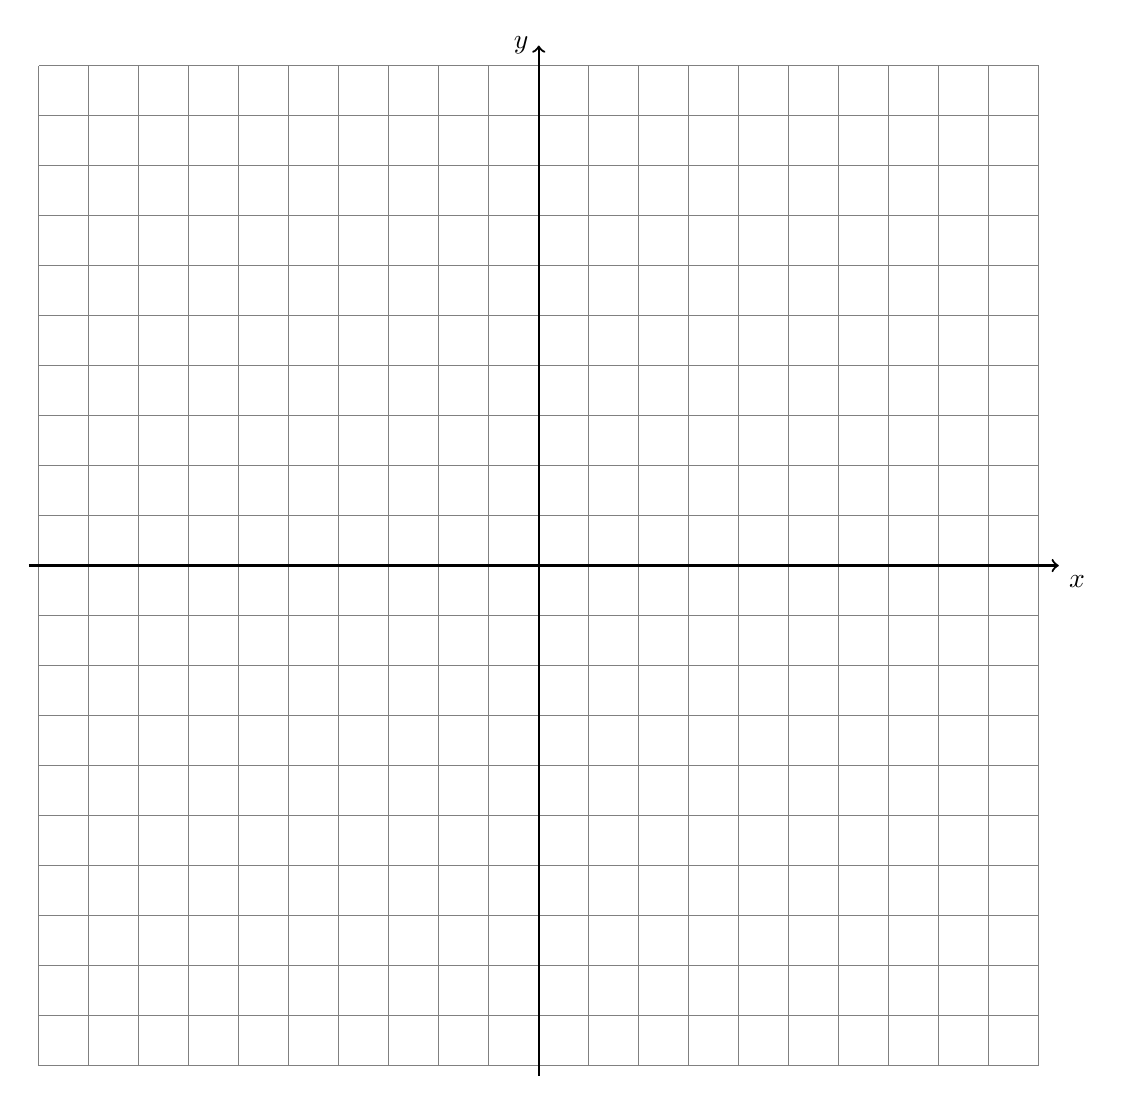
\begin{tikzpicture}[scale=.635]
      \draw [help lines] (-10,-10) grid (10,10);
      \draw [thick, ->] (-10.2,0) -- (10.4,0) node [below right] {$x$};
      \draw [thick, ->] (0,-10.2)--(0,10.4) node [left] {$y$};
    \end{tikzpicture}
    \end{center}

\end{enumerate}
\end{document}